%###########################PRESENTACION##########################################
%Modo presentación
\documentclass[14pt]{beamer}

%Modo handout
%\documentclass[handout,compress]{beamer}
%\usepackage{pgfpages}
%\pgfpagesuselayout{4 on 1}[border shrink=1mm]

\usepackage{graphicx,pstricks}
\usepackage{beamerthemeCambridgeUS}
\usepackage{subfig}
\usepackage{tikz}
\usepackage{amsmath}
\usepackage{hyperref}

\graphicspath{{G:/My Drive/FIGURAS/}}
\setbeamercovered{transparent}

\title[GIS]{ANÁLISIS GEOESPACIAL}
\author[Edier Aristizábal]{Edier V. Aristizábal G.}
\institute{\emph{evaristizabalg@unal.edu.co}}
\date{\tiny{(Versión:\today)}}
\usepackage{textpos}

\addtobeamertemplate{headline}{}{%
	\begin{textblock*}{2mm}(.9\textwidth,0cm)
	\hfill
\includegraphics[height=1cm]{un}
	\end{textblock*}
			}
%############################INICIO#############################################
\begin{document}
\begin{frame}
\titlepage
\centering
	
\includegraphics[width=5cm]{unal}\hspace*{4.75cm}~%
   	
\includegraphics[width=2cm]{logo3}
\end{frame}
 %#############################SLIDE
\begin{frame}
\frametitle{Sistemas de Información Geográfica}
\framesubtitle{\emph {Elemento para analizar, presentar e interpretar datos espaciales}}
  \begin{figure}
    \centering
    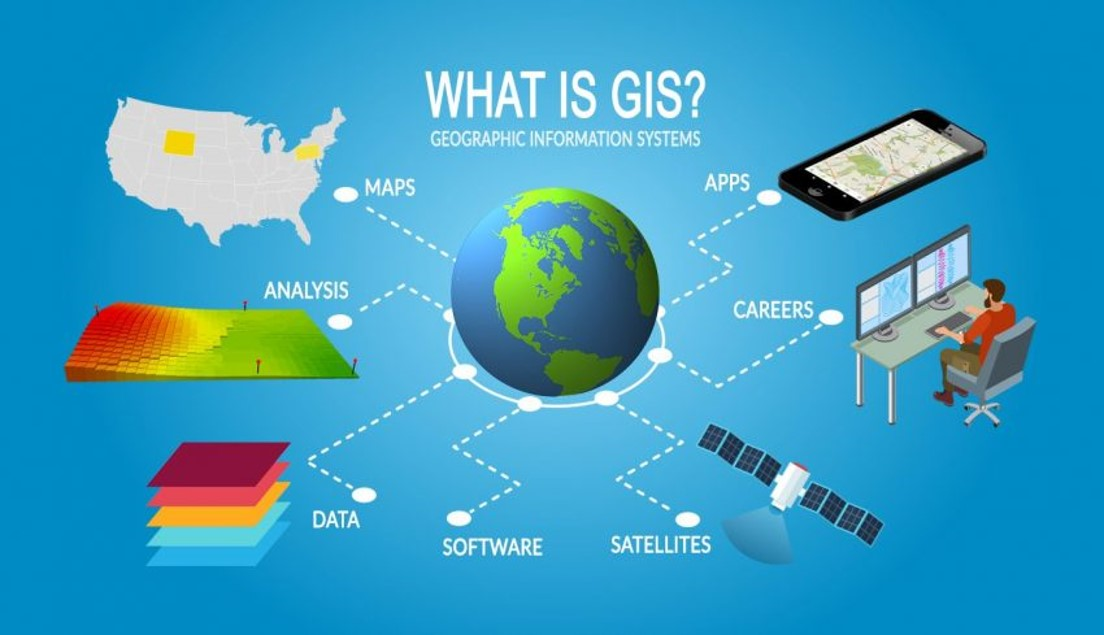
\includegraphics[height=.7\textheight]{gis}
    %\caption{This is the caption.}
  \end{figure}
\end{frame}
%################################SLIDE
\begin{frame}\frametitle{Evolución de GIS}
\begin{columns}
		\begin{column}{.48\linewidth}
			\begin{figure}
				\includegraphics[width=4cm]{colera}\\
			\end{figure}
		\end{column}
		\begin{column}{.48\linewidth}
			\begin{figure}
				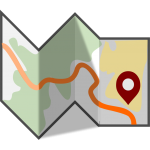
\includegraphics[width=2cm]{webgi}\\
			\end{figure}
		\end{column}
	\end{columns}
	\begin{columns}
		\begin{column}{.48\linewidth}
			\begin{figure}
				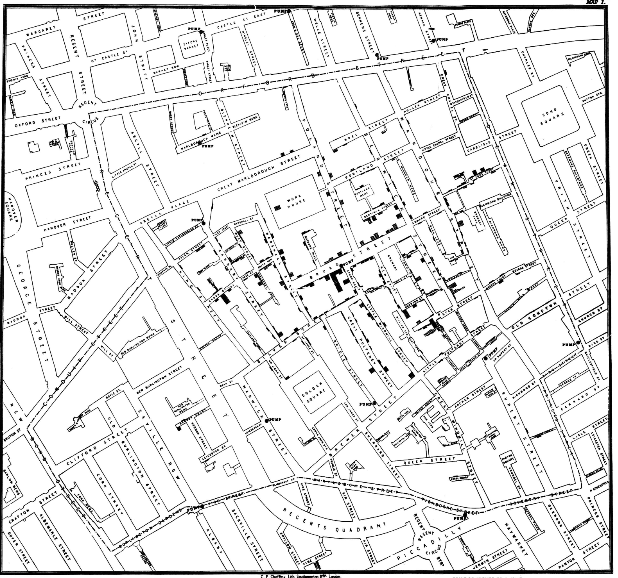
\includegraphics[width=2cm]{snow}\\
			\end{figure}
\scriptsize{In 1854\, cholera hit the city of London, England. No one knew where the disease started. So, British physician \emph{John Snow} started mapping the outbreak. But he also mapped out roads, property boundaries and water lines.}
		\end{column}
		\begin{column}{.48\linewidth}
			\begin{figure}
				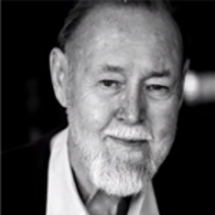
\includegraphics[width=2cm]{tomlinson}\\
			\end{figure}
\scriptsize{In 1968, \emph{Roger Tomlinson} coined the term “GIS” in his paper “A Geographic Information System for Regional Planning“. In 2014, Roger Tomlinson later passed away and will always be remembered as the \emph{father of GIS}.}
		\end{column}
	\end{columns}
\end{frame}
%###############################SLIDE
\begin{frame}
  \begin{figure}
    \centering
    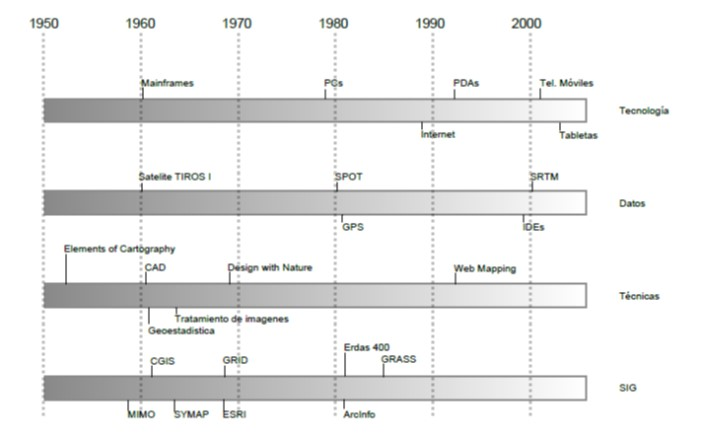
\includegraphics[height=.7\textheight]{historia}
    %\caption{This is the caption.}
  \end{figure}
\end{frame}
%################################SLIDE
\begin{frame}
\frametitle{Componentes de un SIG}
\framesubtitle{Data \& Hardware \& Software}
  \begin{figure}
    \centering
    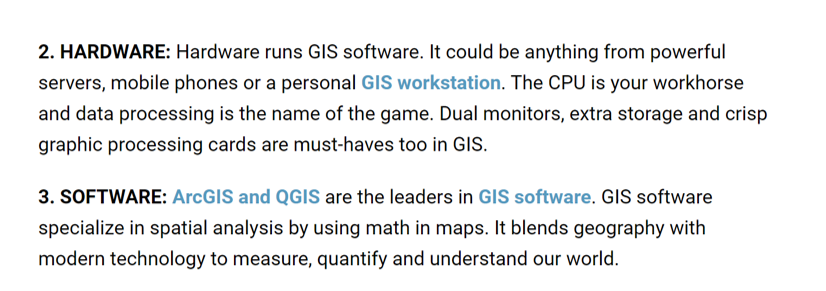
\includegraphics[width=10cm]{component2}
    %\caption{This is the caption.}
   \end{figure}
\begin{columns}
		\begin{column}{.33\linewidth}
		 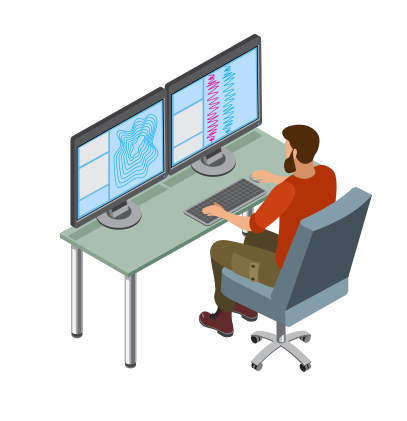
\includegraphics[height=.4\textheight]{component3}
		\end{column}
		\begin{column}{.33\linewidth}
			 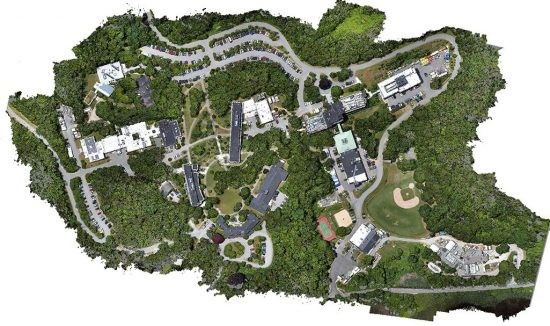
\includegraphics[height=.2\textheight]{component4}
		\end{column}
		\begin{column}{.33\linewidth}
			 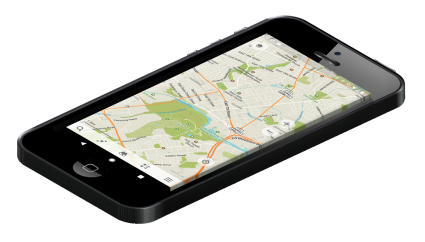
\includegraphics[height=.3\textheight]{component5}
		\end{column}
	\end{columns}
\end{frame}
%################################SLIDE
\begin{frame}
\frametitle{Hardware}
  \begin{figure}
    \centering
    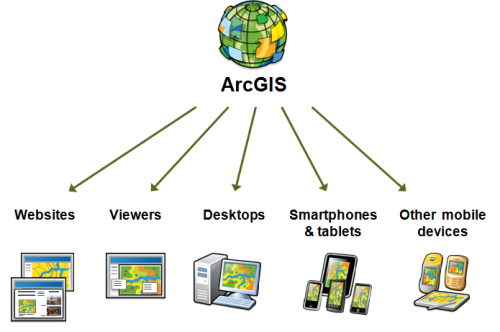
\includegraphics[height=.8\textheight]{web}
    %\caption{This is the caption.}
  \end{figure}
\end{frame}
%################################SLIDE
\begin{frame}
\frametitle{Software}
  \begin{figure}
    \centering
    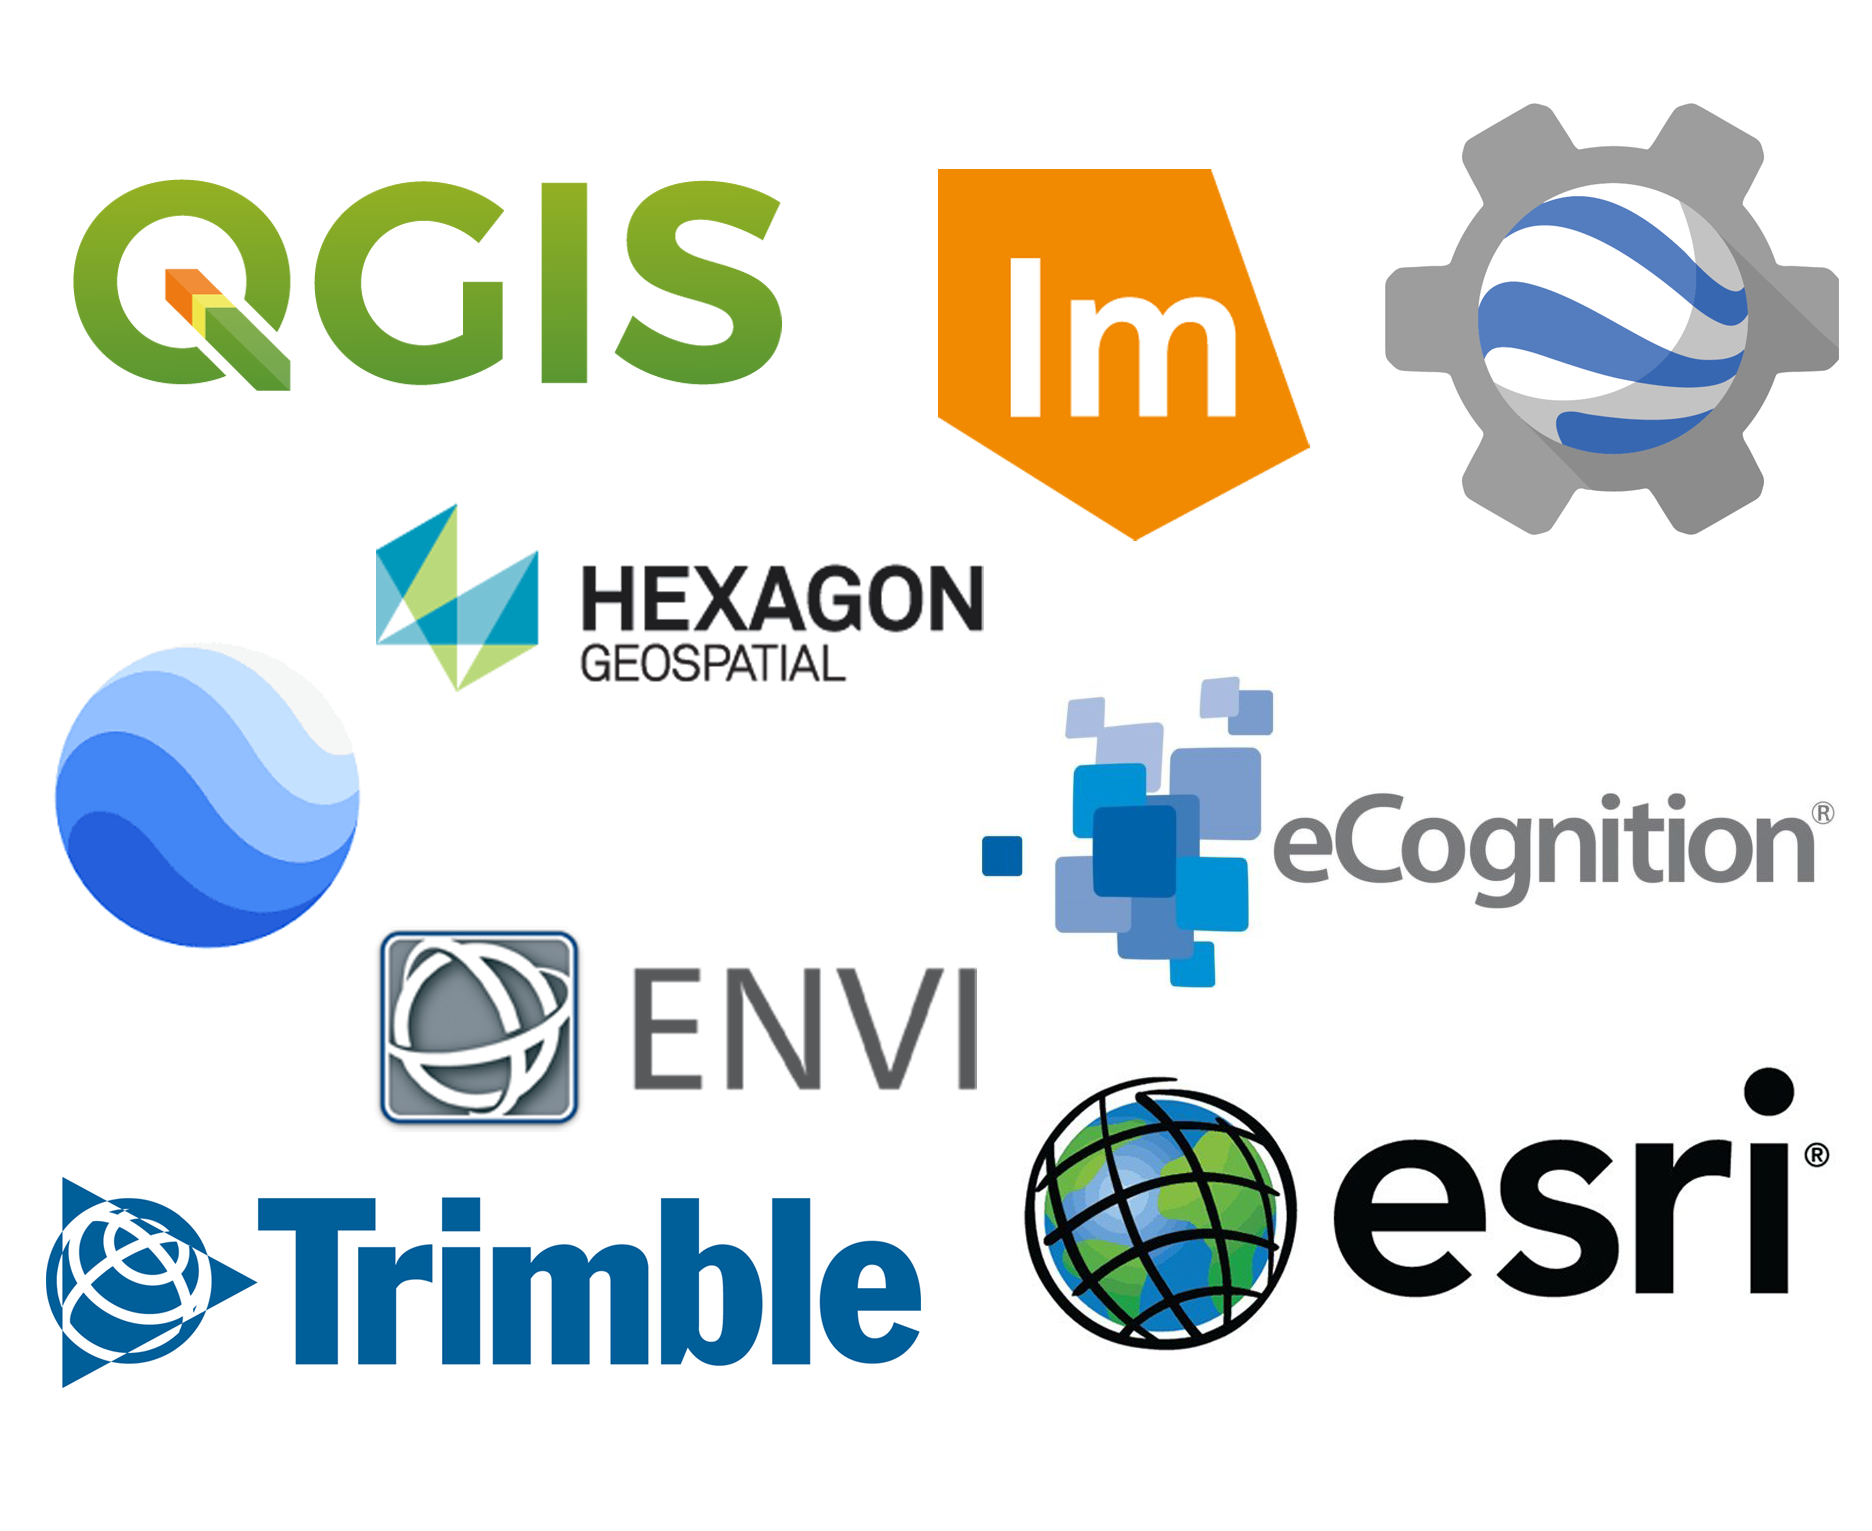
\includegraphics[height=.8\textheight]{Softwarelogos2}
    %\caption{This is the caption.}
  \end{figure}
\end{frame}
%################################SLIDE
\begin{frame}
\frametitle{Software}
  \begin{figure}
    \centering
    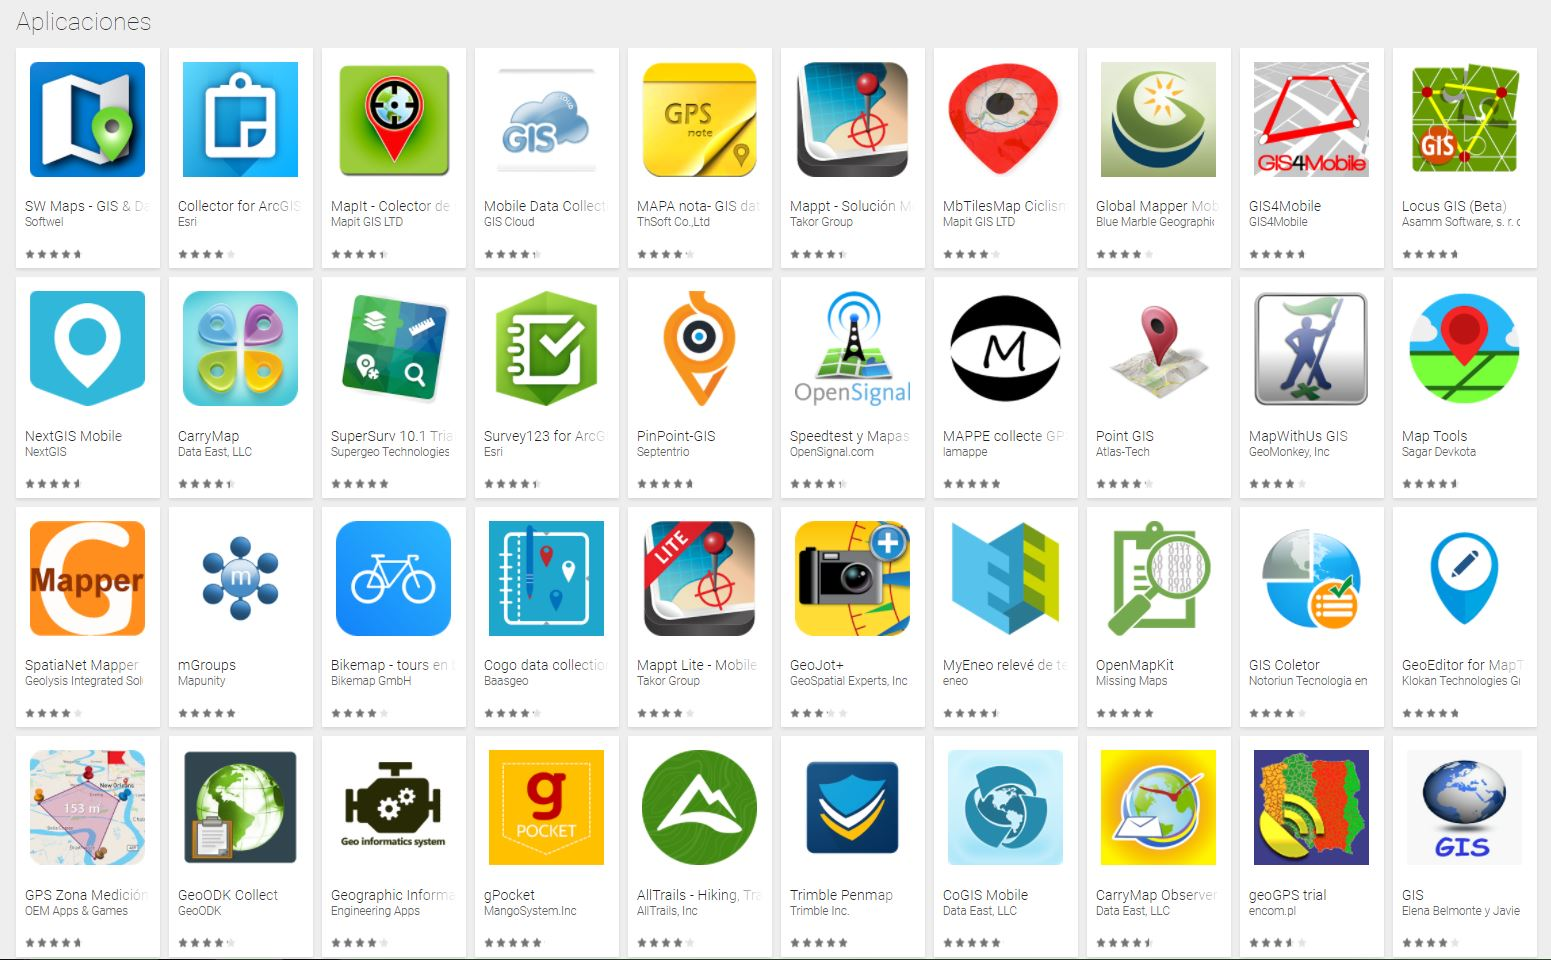
\includegraphics[height=.8\textheight]{android}
    %\caption{This is the caption.}
  \end{figure}
\end{frame}
%###############################SLIDE
\begin{frame}
\frametitle{Componentes de un SIG}
\framesubtitle{Data \& Hardware \& Software}
  \begin{figure}
    \centering
    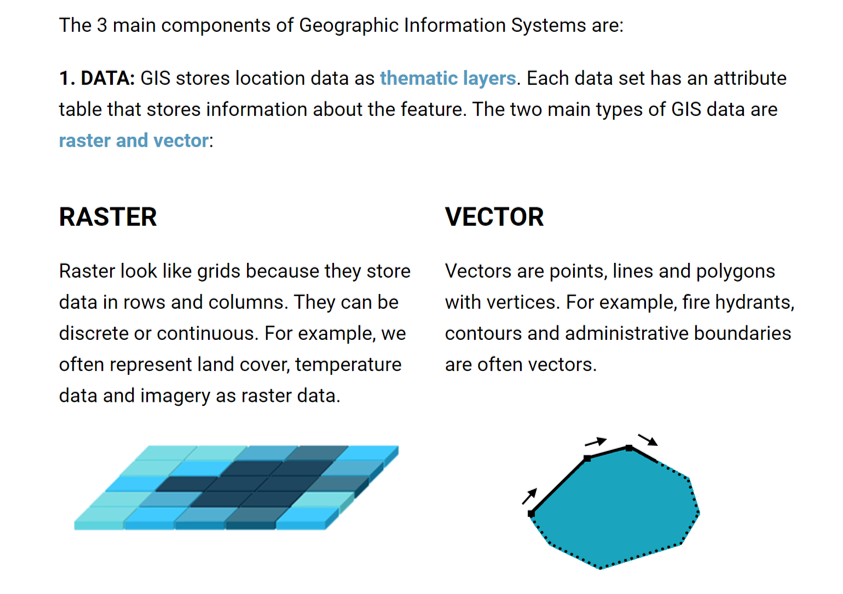
\includegraphics[height=.7\textheight]{component}
    %\caption{This is the caption.}
  \end{figure}
\end{frame}
%###############################SLIDE
\begin{frame}
\frametitle{Geospatial Data}
  \begin{figure}
    \centering
    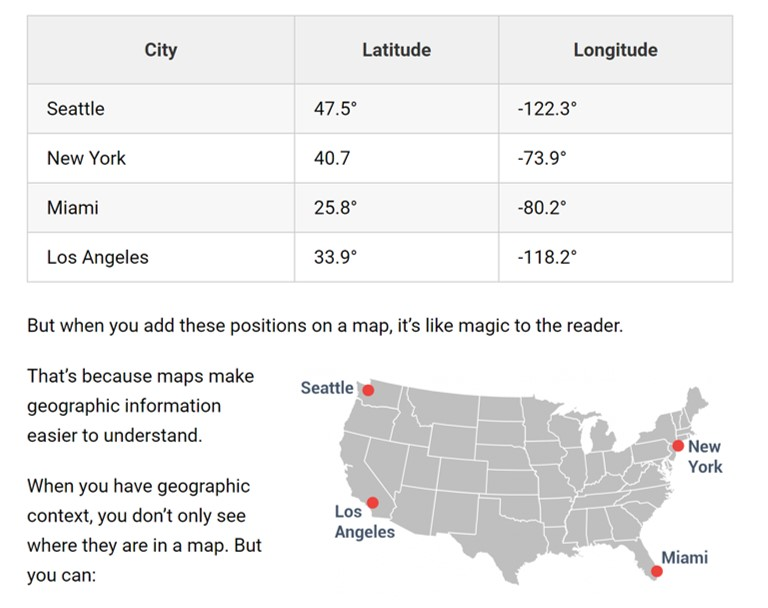
\includegraphics[height=.7\textheight]{table}
    %\caption{This is the caption.}
  \end{figure}
\end{frame}
%################################SLIDE
\begin{frame}
\frametitle{Geospatial Data}
\scriptsize{Geospatial data is data about objects, events, or phenomena that have a location on the surface of the earth, including location information (usually coordinates on the earth), attribute information (the characteristics of the object, event, or phenomena concerned), and often also temporal information (the time or life span at which the location and attributes exist).}
%\framesubtitle{}
  \begin{figure}
    \centering
    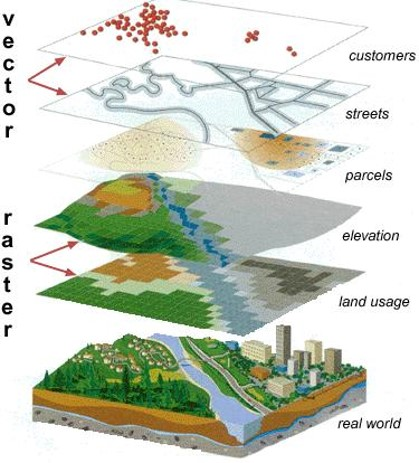
\includegraphics[height=.7\textheight]{vector}
    %\caption{This is the caption.}
  \end{figure}
\end{frame}
%################################SLIDE
\begin{frame}
\frametitle{GIS Data Models}
  \begin{figure}
    \centering
    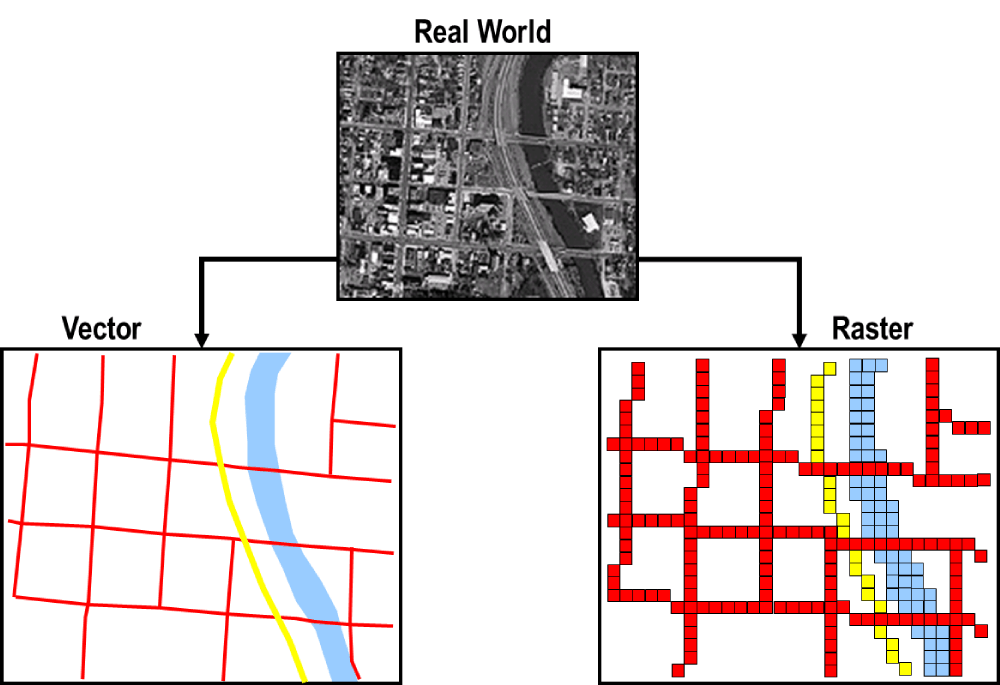
\includegraphics[height=.7\textheight]{gis_data_models}
  \end{figure}
  \tiny{\url{https://transportgeography.org/?page_id=6748}}
\end{frame}
%################################SLIDE
\begin{frame}
%\framesubtitle{}
  \begin{figure}
    \centering
    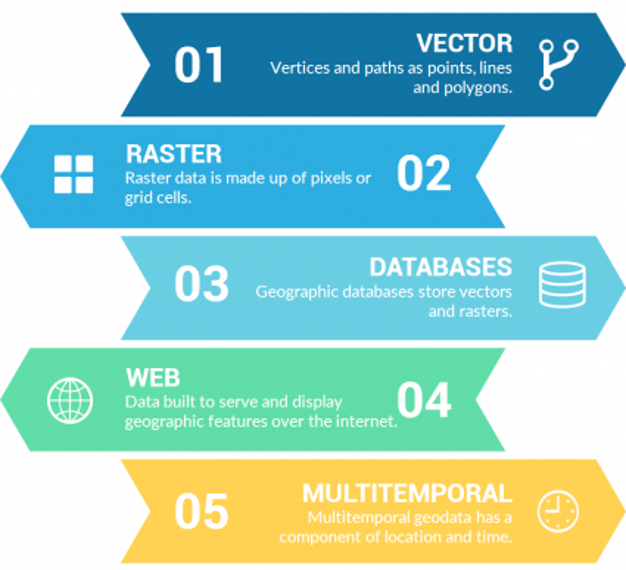
\includegraphics[height=.7\textheight]{data}
    %\caption{This is the caption.}
  \end{figure}
\end{frame}
%################################SLIDE
\begin{frame}
\frametitle{Data}
  \begin{figure}
    \centering
    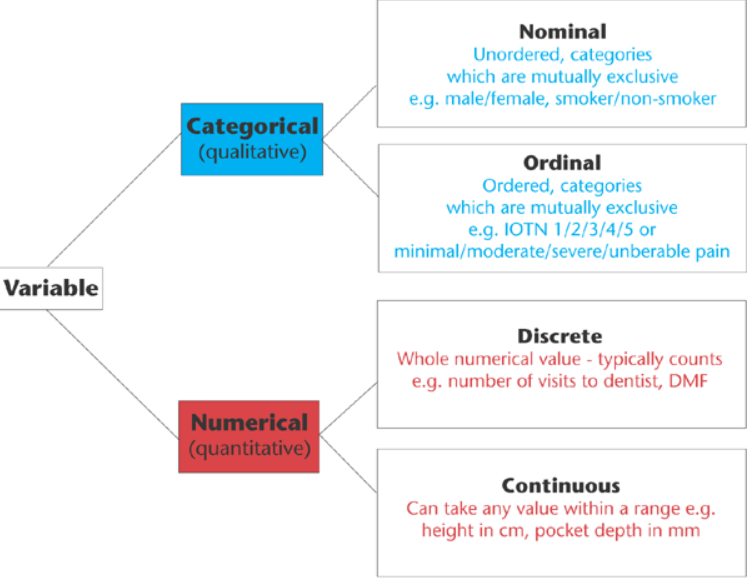
\includegraphics[height=.6\textheight]{type}
    %\caption{This is the caption.}
  \end{figure}
\end{frame}
%################################SLIDE
\begin{frame}
\frametitle{Vector}
  \begin{figure}
    \centering
    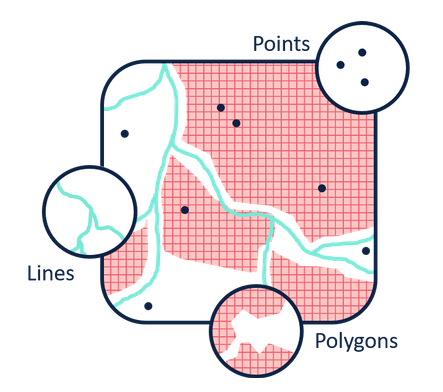
\includegraphics[height=.75\textheight]{vector_data}
  \end{figure}
\tiny{\url{https://datenlage.blog/2019/06/08/geospatial-data-1/}}
\end{frame}
%################################SLIDE
\begin{frame}
\frametitle{Vector}
  \begin{figure}
    \centering
    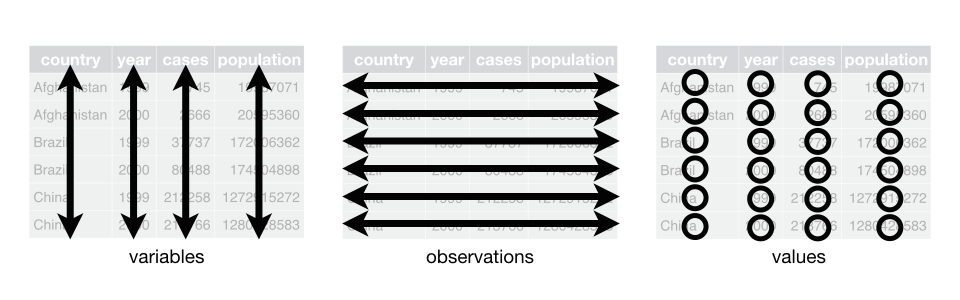
\includegraphics[height=.4\textheight]{data2}
    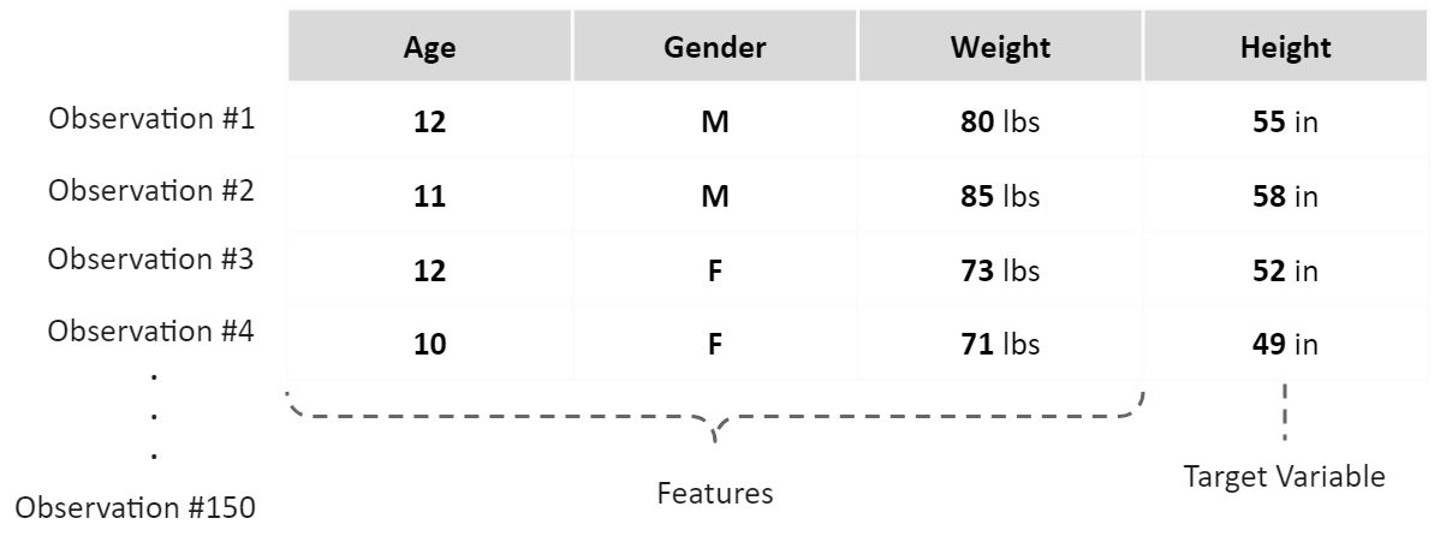
\includegraphics[height=.4\textheight]{data3}
  \end{figure}
\end{frame}
%################################SLIDE
\begin{frame}
\frametitle{Raster}
  \begin{columns}
		\begin{column}{.33\linewidth}
		 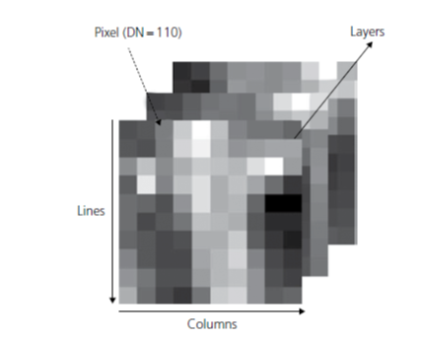
\includegraphics[height=.4\textheight]{celda}
		\end{column}
		\begin{column}{.33\linewidth}
			 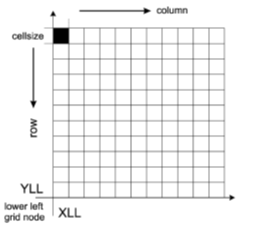
\includegraphics[height=.45\textheight]{rast2}
		\end{column}
		\begin{column}{.33\linewidth}
			 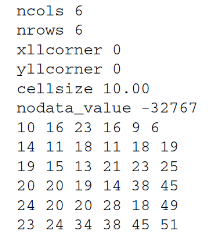
\includegraphics[height=.5\textheight]{rast3}
		\end{column}
	\end{columns}\vfill
\tiny{Wood, J. (2009). Geomorphometry - Concepts, Software, Applications. In Developments in Soil Science (Vol. 33). https://doi.org/10.1016/S0166-2481(08)00010-X}
\end{frame}
%################################SLIDE
\begin{frame}
\frametitle{Raster Continuos}
\scriptsize{Continuous rasters (non-discrete) are grid cells with gradual changing data such as elevation, temperature or an aerial photograph. A continuous raster surface can be derived from a fixed registration point. For example, digital elevation models use sea level as a registration point. Each cell represents a value above or below sea level.}
%\framesubtitle{}
  \begin{figure}
    \centering
    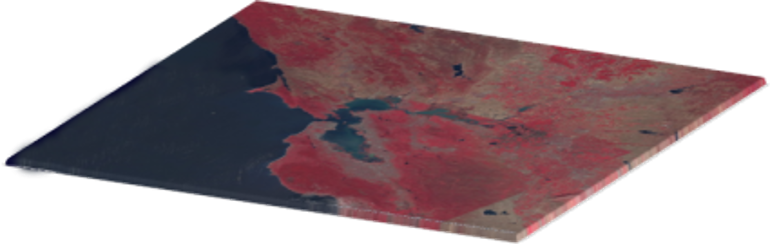
\includegraphics[height=.4\textheight]{conraster}
    %\caption{This is the caption.}
  \end{figure}
\end{frame}
%################################SLIDE
\begin{frame}
\frametitle{Raster Discretos}
\scriptsize{Discrete rasters have distinct themes or categories. For example, one grid cell represents a land cover class or a soil type.In a discrete raster land cover/use map, you can distinguish each thematic class. Each class can be discretely defined where it begins and ends. In other words, each land cover cell is definable and it fills the entire area of the cell.Discrete data usually consists of integers to represent classes.}
%\framesubtitle{}
  \begin{figure}
    \centering
    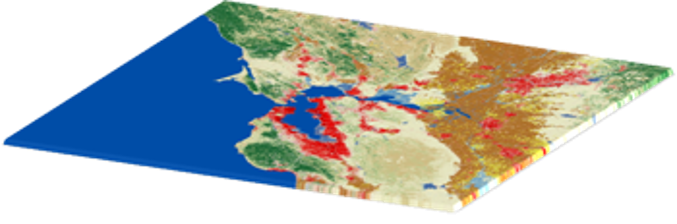
\includegraphics[height=.4\textheight]{disraster}
    %\caption{This is the caption.}
  \end{figure}
\end{frame}
%################################SLIDE
\begin{frame}
\frametitle{Formatos}
%\framesubtitle{}
%\scriptsize{}
  \begin{figure}
    \centering
    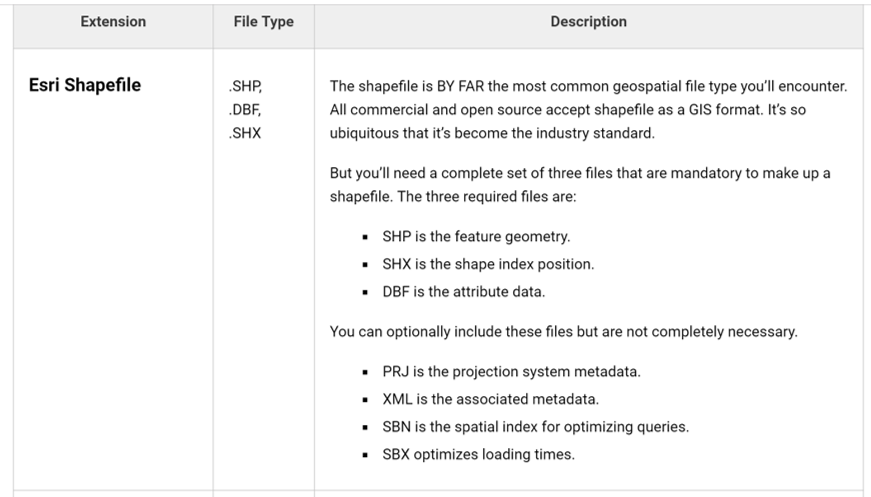
\includegraphics[height=.7\textheight]{shape}
    %\caption{This is the caption.}
  \end{figure}
\end{frame}
%################################SLIDE
\begin{frame}
\frametitle{Vector}
%\framesubtitle{}
%\scriptsize{}
  \begin{figure}
    \centering
    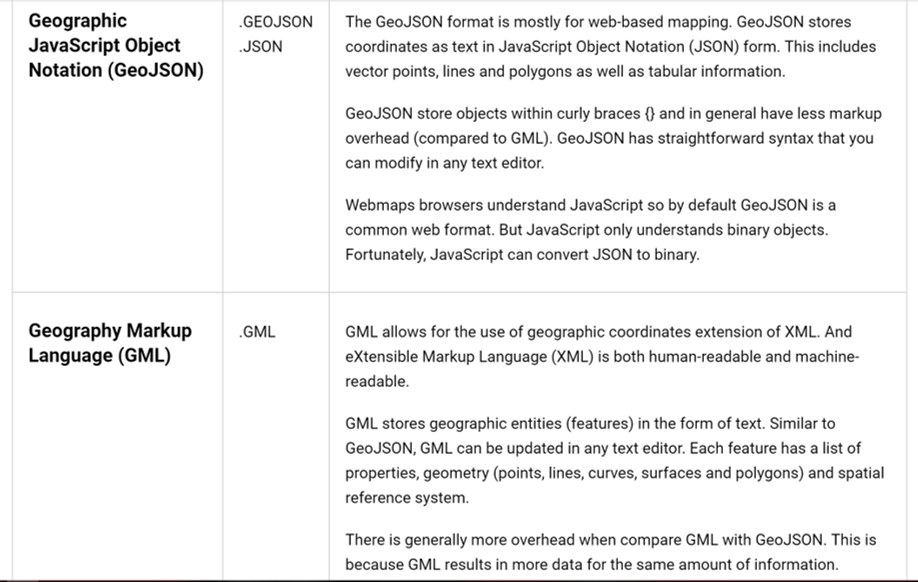
\includegraphics[height=.7\textheight]{json}
    %\caption{This is the caption.}
  \end{figure}
\end{frame}
%################################SLIDE
\begin{frame}
\frametitle{Vector}
%\framesubtitle{}
%\scriptsize{}
  \begin{figure}
    \centering
    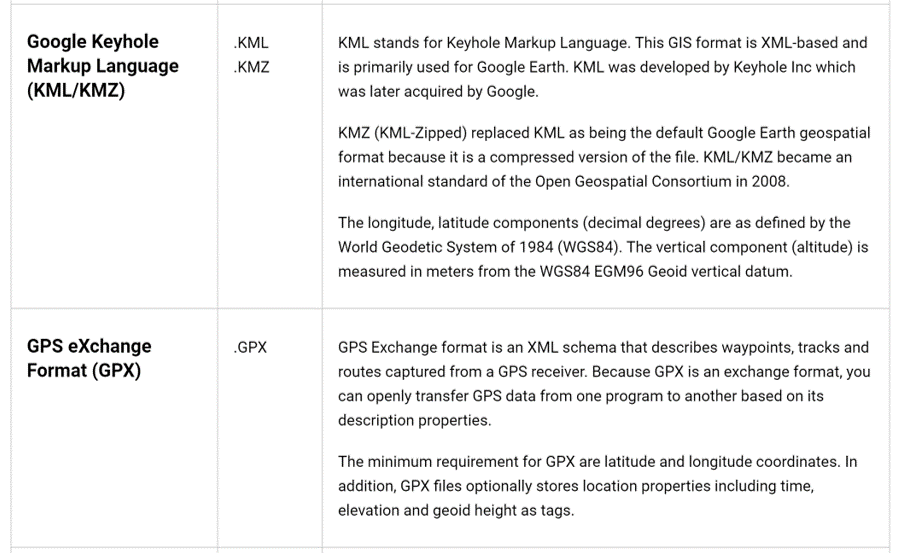
\includegraphics[height=.7\textheight]{kml}
    %\caption{This is the caption.}
  \end{figure}
\end{frame}
%################################SLIDE
\begin{frame}
\frametitle{Raster}
%\framesubtitle{}
%\scriptsize{}
  \begin{figure}
    \centering
    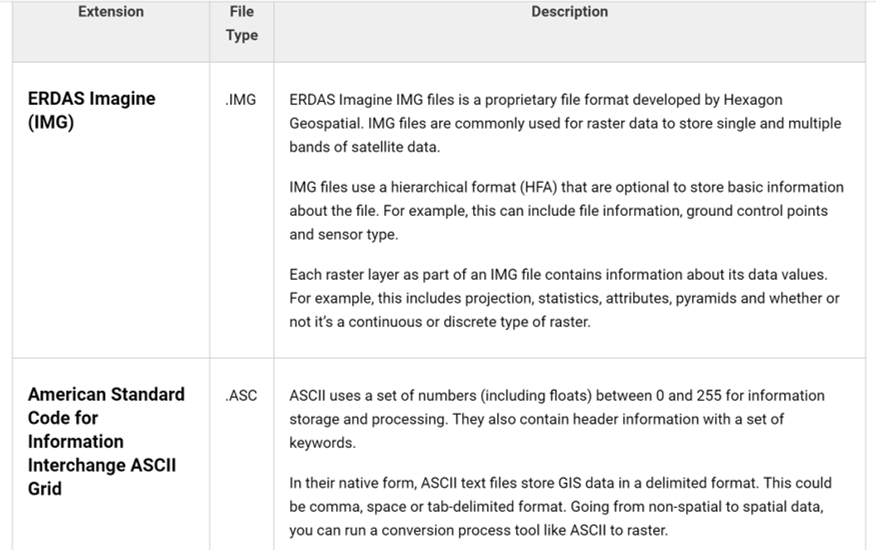
\includegraphics[height=.7\textheight]{raster}
    %\caption{This is the caption.}
  \end{figure}
\end{frame}
%################################SLIDE
\begin{frame}
\frametitle{Raster}
%\framesubtitle{}
%\scriptsize{}
  \begin{figure}
    \centering
    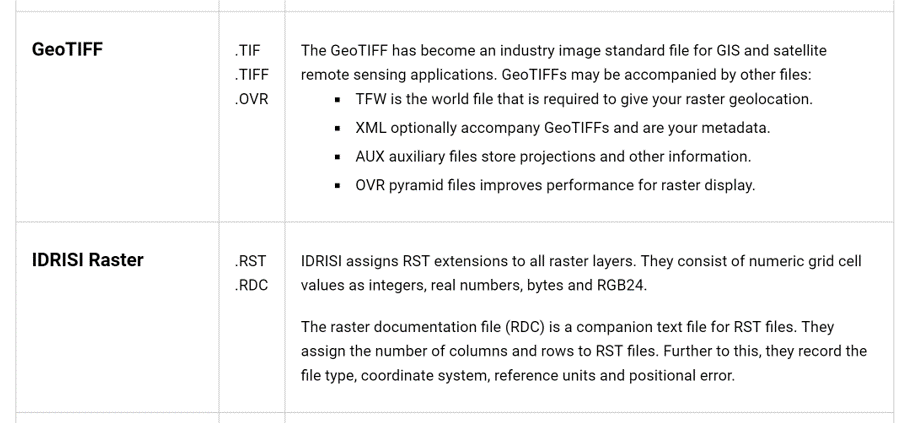
\includegraphics[height=.7\textheight]{tiff}
    %\caption{This is the caption.}
  \end{figure}
\end{frame}
%################################SLIDE
\begin{frame}
\frametitle{Raster}
%\framesubtitle{}
%\scriptsize{}
  \begin{figure}
    \centering
    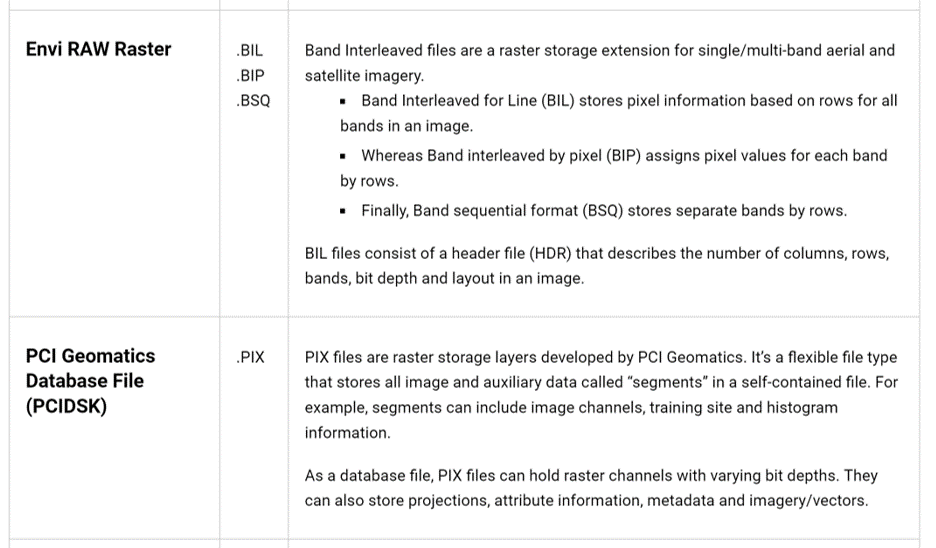
\includegraphics[height=.7\textheight]{bil}
    %\caption{This is the caption.}
  \end{figure}
\end{frame}
%################################SLIDE
\begin{frame}
\frametitle{Raster}
%\framesubtitle{}
%\scriptsize{}
  \begin{figure}
    \centering
    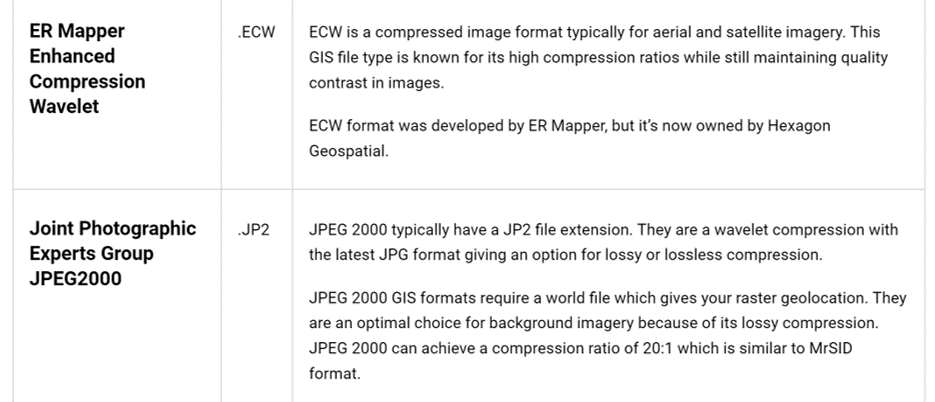
\includegraphics[height=.6\textheight]{ecw}
    %\caption{This is the caption.}
  \end{figure}
\end{frame}
%################################SLIDE
\begin{frame}
\frametitle{Raster}
%\framesubtitle{}
%\scriptsize{}
  \begin{figure}
    \centering
    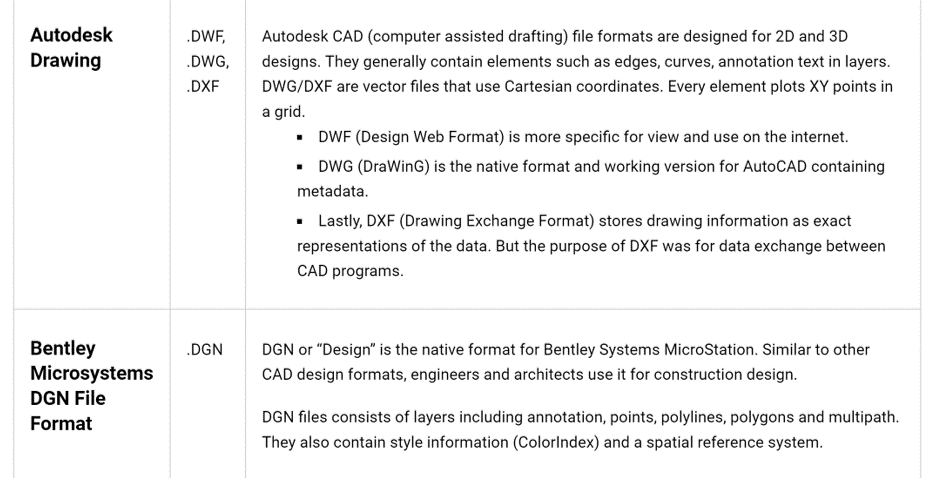
\includegraphics[height=.7\textheight]{dwg}
    %\caption{This is the caption.}
  \end{figure}
\end{frame}
%################################SLIDE
\begin{frame}
\frametitle{Raster}
%\framesubtitle{}
%\scriptsize{}
  \begin{figure}
    \centering
    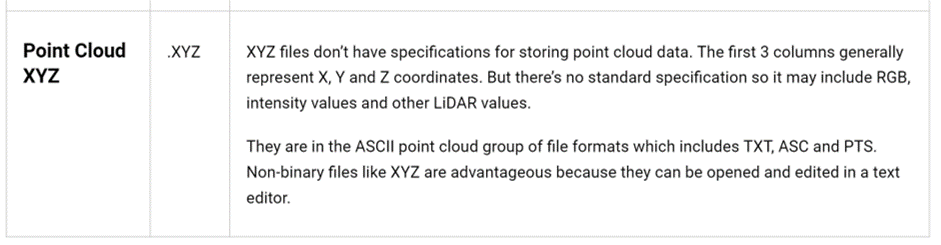
\includegraphics[height=.4\textheight]{xyz}
    %\caption{This is the caption.}
  \end{figure}
\end{frame}
%################################SLIDE
\begin{frame}
\frametitle{Raster}
%\framesubtitle{}
%\scriptsize{}
  \begin{figure}
    \centering
    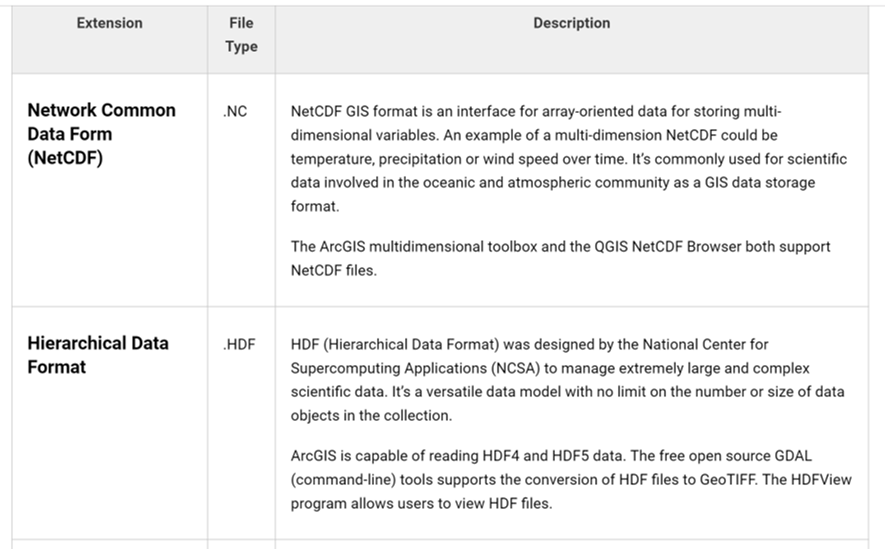
\includegraphics[height=.7\textheight]{nfc}
    %\caption{This is the caption.}
  \end{figure}
\end{frame}
%################################SLIDE
\begin{frame}
\frametitle{\emph{The Earth}}
  \begin{figure}
    \centering
    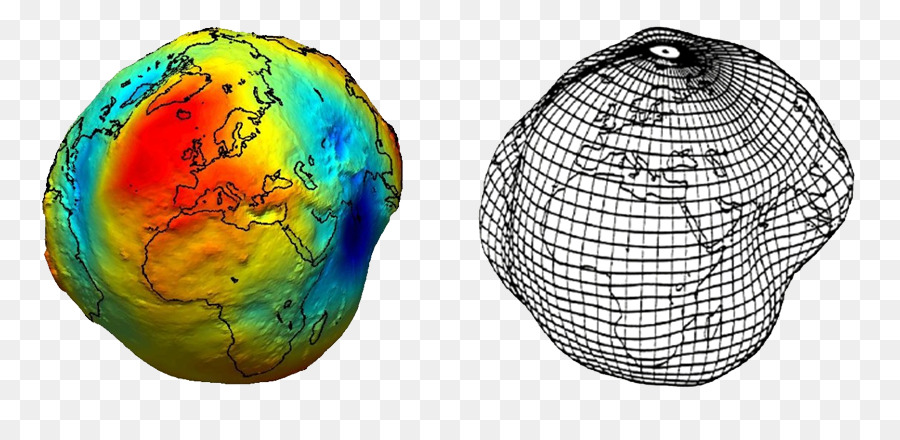
\includegraphics[height=.7\textheight]{earth}
    %\caption{This is the caption.}
  \end{figure}
\end{frame}
%################################SLIDE
\begin{frame}
\frametitle{Geoide}
  \begin{figure}
    \centering
    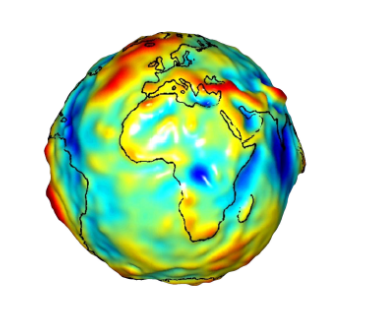
\includegraphics[height=.7\textheight]{geoide}
    %\caption{This is the caption.}
  \end{figure}
\end{frame}
%################################SLIDE
\begin{frame}
\frametitle{Elipsoide}
\framesubtitle{WGS84}
  \begin{figure}
    \centering
    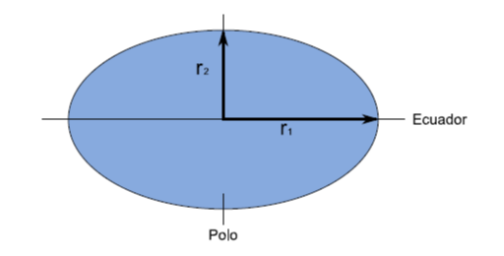
\includegraphics[height=.7\textheight]{elipsoide}
    %\caption{This is the caption.}
  \end{figure}
\end{frame}
%################################SLIDE
\begin{frame}
\frametitle{Elipsoide \& Geoide}
\framesubtitle{Datum geodésico}
  \begin{figure}
    \centering
    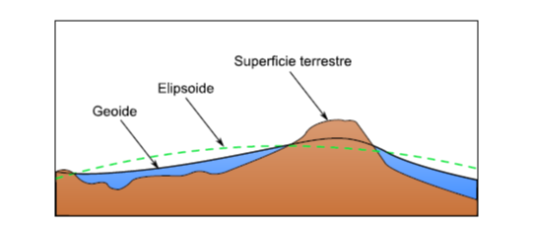
\includegraphics[height=.6\textheight]{geoide2}
    %\caption{This is the caption.}
  \end{figure}
\end{frame}
%################################SLIDE
\begin{frame}
\frametitle{Coordenadas Geográficas}
%\framesubtitle{}
  \begin{figure}
    \centering
    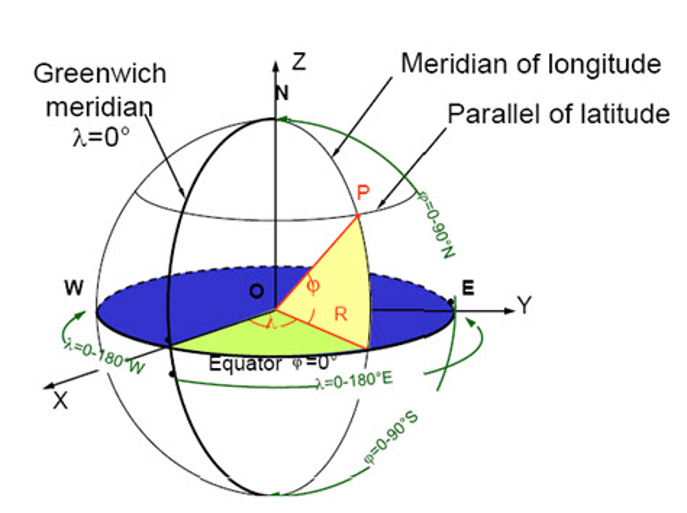
\includegraphics[height=.7\textheight]{coordenadas}
    %\caption{This is the caption.}
  \end{figure}
\end{frame}
%################################SLIDE
\begin{frame}
\frametitle{Proyección a Coordenadas Planas}
\framesubtitle{\emph{You can’t represent Earth’s surface in two dimensions without distortion}}
\scriptsize{Similarly, a map projection is a method by which cartographers translates a sphere or globe into a two-dimensional representation. In other words, a map projection systematically renders a 3D ellipsoid (or spheroid) of Earth to a 2D map surface. Because you can’t display 3D surfaces perfectly in two dimensions, distortions always occur. For example, map projections distort distance, direction, scale and area.}
  \begin{figure}
    \centering
    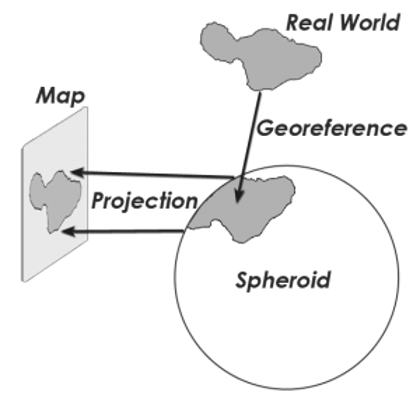
\includegraphics[height=.6\textheight]{projec}
    %\caption{This is the caption.}
  \end{figure}
\end{frame}
%################################SLIDE
\begin{frame}
\frametitle{Proyección Cartográfica}
%\framesubtitle{}
  \begin{figure}
    \centering
    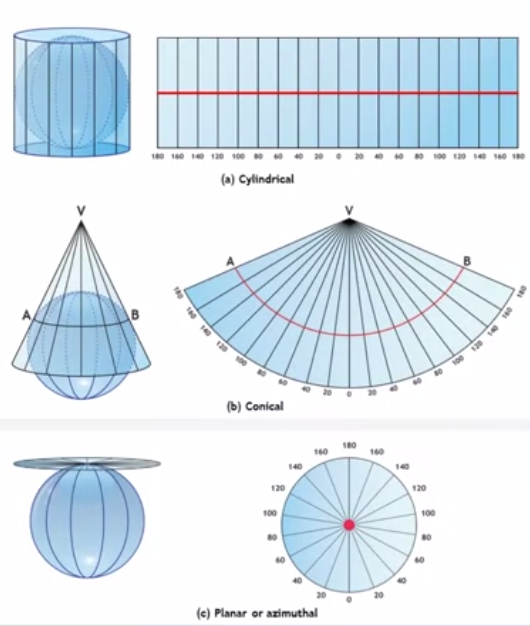
\includegraphics[height=.8\textheight]{proy}
    %\caption{This is the caption.}
  \end{figure}
\end{frame}
%################################SLIDE
\begin{frame}
\frametitle{Proyección Cilíndrica}
%\framesubtitle{}
  \begin{figure}
    \centering
    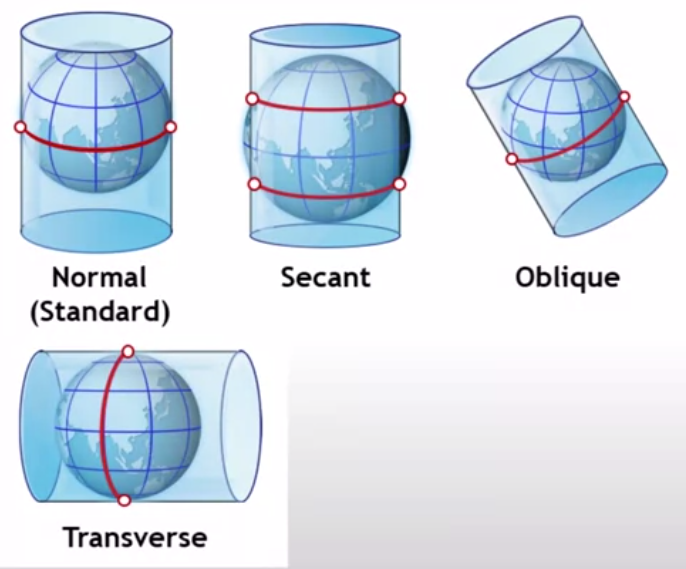
\includegraphics[height=.8\textheight]{cilindrica}
    %\caption{This is the caption.}
  \end{figure}
\end{frame}
%################################SLIDE
\begin{frame}
\frametitle{Proyección Cónica}
%\framesubtitle{}
  \begin{figure}
    \centering
    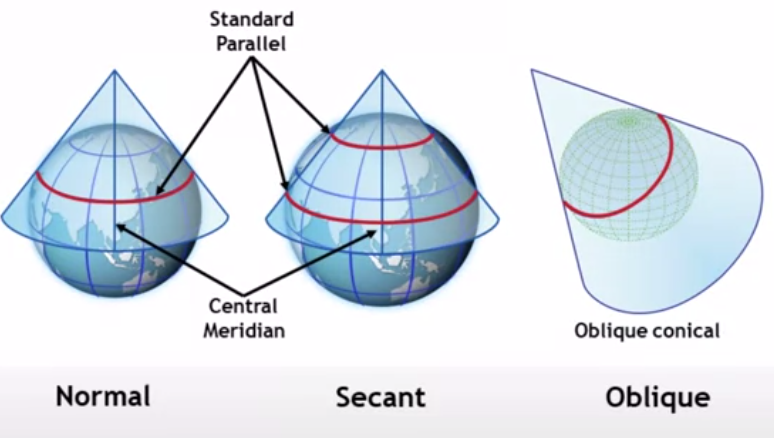
\includegraphics[height=.8\textheight]{conical}
    %\caption{This is the caption.}
  \end{figure}
\end{frame}
%################################SLIDE
\begin{frame}
\frametitle{Proyección Planar}
%\framesubtitle{}
  \begin{figure}
    \centering
    \includegraphics[height=.8\textheight]{Planar}
    %\caption{This is the caption.}
  \end{figure}
\end{frame}
%################################SLIDE
\begin{frame}
\frametitle{Proyección Cartográfica}
%\framesubtitle{}
  \begin{figure}
    \centering
    \includegraphics[height=.7\textheight]{proye}
    %\caption{This is the caption.}
  \end{figure}
\end{frame}
%################################SLIDE
\begin{frame}
\frametitle{Universal Transversal Mercator (UTM)}
%\framesubtitle{}
  \begin{figure}
    \centering
    \includegraphics[height=.7\textheight]{utm}
    %\caption{This is the caption.}
  \end{figure}
\end{frame}
%################################SLIDE
\begin{frame}
\frametitle{Proyección Conforme de Gauss}
%\framesubtitle{}
  \begin{figure}
    \centering
    \includegraphics[height=.8\textheight]{gauss}
    %\caption{This is the caption.}
  \end{figure}
\end{frame}
%################################SLIDE
\begin{frame}
\frametitle{Proyección Conforme de Gauss}
%\framesubtitle{}
  \begin{figure}
    \centering
    \includegraphics[height=.7\textheight]{gauss2}
    %\caption{This is the caption.}
  \end{figure}
\end{frame}
%################################SLIDE
\begin{frame}
\frametitle{Spatial Reference System Identifier (SRID)}
\scriptsize{Un SRID, Identificador de Referencia Espacial, es un identificador estándar único que hace referencia a un Sistema de Coordenadas concreto. Cada código, por tanto, se asocia de forma exclusiva a un Sistema de Coordenadas.}
%\framesubtitle{}
  \begin{figure}
    \centering
    \includegraphics[height=.6\textheight]{epsg}
    %\caption{This is the caption.}
  \end{figure}
\url{https://www.spatialreference.org/}
\end{frame}
%################################SLIDE
\begin{frame}
\frametitle{The True Size of...}
\framesubtitle{\url{https://thetruesize.com}}
  \begin{figure}
  \centering
    \includegraphics[height=0.8\textheight]{truesize}
\tiny{}
  \end{figure}
\end{frame}
%################################SLIDE
\begin{frame}
\begin{figure}[]
 \centering
  \begin{picture}(10,10)  
    \put(-170,-110){\includegraphics[scale=0.18]{dsm2}}
    \put(-140,60){\color{black}{\huge Digital Elevation Models}}
    \put(-170,-127) {\tiny{https://medium.com/on-location/from-points-to-pixels-creating-digital-elevation-models-from-open-topography-point-clouds}}
    \end{picture}
\end{figure}
\end{frame}
%################################SLIDE
\begin{frame}
\frametitle{DEM}
%\framesubtitle{}
\begin{columns}
		\begin{column}{.30\linewidth}
		 \includegraphics[width=4cm]{dtm3}
		\end{column}
		\begin{column}{.70\linewidth}
			 \includegraphics[width=8cm]{dtm2}
		\end{column}
	\end{columns}
\end{frame}
%################################SLIDE
\begin{frame}
\frametitle{DEM}
  \begin{figure}
    \centering
    \includegraphics[height=.5\textheight]{dtm}
    %\caption{This is the caption.}
  \end{figure}
\end{frame}
%################################SLIDE
\begin{frame}
\frametitle{Modelos Digitales de Elevación (DEM)}
  \begin{figure}
    \centering
    \includegraphics[height=.5\textheight]{dsm}\vfill
\tiny{Arbeck / CC BY (https://creativecommons.org/licenses/by/4.0)}
  \end{figure}
\end{frame}
%################################SLIDE
\begin{frame}
\frametitle{DTM}
%\framesubtitle{}
  \begin{figure}
    \centering
    \includegraphics[width=2cm]{dem3}
    %\caption{This is the caption.}
   \end{figure}
\begin{columns}
		\begin{column}{.5\linewidth}
		 \includegraphics[width=4cm]{tin}
		\end{column}
		\begin{column}{.5\linewidth}
			 \includegraphics[width=4cm]{rast1}
		\end{column}
\end{columns}
\end{frame}
%################################SLIDE
\begin{frame}
  \begin{figure}
    \centering
    \includegraphics[height=.8\textheight]{dtm5}
    %\caption{This is the caption.}
  \end{figure}
\end{frame}
%################################SLIDE
\begin{frame}
  \begin{figure}
    \centering
    \includegraphics[height=.8\textheight]{dtm6}
    %\caption{This is the caption.}
  \end{figure}
\end{frame}
%################################SLIDE
\begin{frame}
\frametitle{Geomorfometría}
  \begin{figure}
    \centering
    \includegraphics[height=.7\textheight]{geomor}
    %\caption{This is the caption.}
  \end{figure}
\end{frame}
%################################SLIDE
\begin{frame}
  \begin{figure}
    \centering
    \includegraphics[height=.8\textheight]{indices}
    %\caption{This is the caption.}
  \end{figure}
\end{frame}
%################################SLIDE
\begin{frame}
  \begin{figure}
    \centering
    \includegraphics[height=.8\textheight]{indice1}
    %\caption{This is the caption.}
  \end{figure}
\end{frame}
%################################SLIDE
\begin{frame}
  \begin{figure}
    \centering
    \includegraphics[height=.7\textheight]{indice3}
    %\caption{This is the caption.}
  \end{figure}
\end{frame}
%################################SLIDE
\begin{frame}
  \begin{figure}
    \centering
    \includegraphics[height=.9\textheight]{indice4}
    %\caption{This is the caption.}
  \end{figure}
\end{frame}
%################################SLIDE
\begin{frame}
\frametitle{Pendiente}
  \begin{figure}
    \centering
    \includegraphics[height=.9\textheight]{pend}
    %\caption{This is the caption.}
  \end{figure}
\end{frame}
%################################SLIDE
\begin{frame}
\frametitle{Curvatura}
  \begin{figure}
    \centering
    \includegraphics[height=.7\textheight]{curv}
    %\caption{This is the caption.}
  \end{figure}
\end{frame}
%################################SLIDE
\begin{frame}
%\framesubtitle{}
\begin{columns}
		\begin{column}{.50\linewidth}
		 \includegraphics[width=6cm]{curv1}
		\end{column}
		\begin{column}{.50\linewidth}
			 \includegraphics[width=6cm]{curv2}
		\end{column}
	\end{columns}
\end{frame}
%################################SLIDE
\begin{frame}
\frametitle{Perfiles}
  \begin{figure}
    \centering
    \includegraphics[height=.7\textheight]{profile}
    %\caption{This is the caption.}
  \end{figure}
\end{frame}
%################################SLIDE
\begin{frame}
\frametitle{Indices morfométricos}
  \begin{figure}
    \centering
    \includegraphics[height=.8\textheight]{indicestabla}
    %\caption{This is the caption.}
  \end{figure}
\end{frame}
%################################SLIDE
\begin{frame}
  \begin{figure}
    \centering
    \includegraphics[height=.8\textheight]{melton}
    %\caption{This is the caption.}
  \end{figure}
\tiny{Fuente: Wilford et al. (2004)}
\end{frame}
%################################SLIDE
\begin{frame}
\frametitle{Perfiles longitudinales}
  \begin{figure}
    \centering
    \includegraphics[height=.6\textheight]{long}
    %\caption{This is the caption.}
  \end{figure}
\tiny{}
\end{frame}
%################################SLIDE
\begin{frame}
  \begin{figure}
    \centering
    \includegraphics[height=.7\textheight]{hack}
    %\caption{This is the caption.}
  \end{figure}
\tiny{}
\end{frame}
%################################SLIDE
\begin{frame}
\frametitle{Curva hipsométrica}
  \begin{figure}
    \centering
    \includegraphics[height=.82\textheight]{hipsom}
    %\caption{This is the caption.}
  \end{figure}
\tiny{}
\end{frame}
%################################SLIDE
\begin{frame}
\frametitle{Indices tectónicos}
  \begin{figure}
    \centering
    \includegraphics[height=.8\textheight]{tect}
    %\caption{This is the caption.}
  \end{figure}
\tiny{}
\end{frame}
%################################SLIDE
\begin{frame}
  \begin{figure}
    \centering
    \includegraphics[height=.8\textheight]{tect2}
    %\caption{This is the caption.}
  \end{figure}
\tiny{}
\end{frame}
%################################SLIDE
\begin{frame}
\frametitle{Geomorfometría \& Análisis Hidrológico}
  \begin{figure}
    \centering
    \includegraphics[height=.8\textheight]{hidro}
    %\caption{This is the caption.}
  \end{figure}
\end{frame}
%################################SLIDE
\begin{frame}
\frametitle{Tratamiento de imágenes de satélite}
%\framesubtitle{}
\scriptsize{Existen una gran cantidad de procedimientos para el análisis de imágenes de satélite. En este curso nos concentraremos en 4 de ellas:}
\begin{itemize}
\item Pro-procesamiento de imágenes
\item Mejoramiento de imágenes
\item Transformaciones de imágenes
\item Clasificación de imágenes.
\end{itemize}
  \begin{figure}
    \centering
    \includegraphics[height=.4\textheight]{band}
    %\caption{This is the caption.}
  \end{figure}
\end{frame}
%################################SLIDE
\begin{frame}
%\framesubtitle{}
\small{Cualquier imagen adquirida por un sensor remoto presenta una serie de alteraciones radiométricas y geométricas debidas a factores como:}
  \begin{figure}
    \centering
    \includegraphics[height=.7\textheight]{correciones}
    %\caption{This is the caption.}
  \end{figure}
\end{frame}
%################################SLIDE
\begin{frame}
\scriptsize{}
  \begin{figure}
    \centering
    \includegraphics[height=.8\textheight]{calibracion}
    %\caption{This is the caption.}
  \end{figure}
\end{frame}
%################################SLIDE
\begin{frame}
\frametitle{Striping}
\scriptsize{}
  \begin{figure}
    \centering
    \includegraphics[height=.7\textheight]{striping}
    %\caption{This is the caption.}
  \end{figure}
\end{frame}
%################################SLIDE
\begin{frame}
\frametitle{Line Drop}
\scriptsize{}
  \begin{figure}
    \centering
    \includegraphics[height=.7\textheight]{linedrop}
    %\caption{This is the caption.}
  \end{figure}
\end{frame}
%################################SLIDE
\begin{frame}
\frametitle{Bit Error}
\scriptsize{}
  \begin{figure}
    \centering
    \includegraphics[height=.6\textheight]{biterror}
    %\caption{This is the caption.}
  \end{figure}
\end{frame}
%################################SLIDE
\begin{frame}
\scriptsize{}
  \begin{figure}
    \centering
    \includegraphics[height=.7\textheight]{toa}
     \end{figure}
\end{frame}
%################################SLIDE
\begin{frame}
\frametitle{Corrección \& Calibración}
\scriptsize{}
  \begin{figure}
    \centering
    \includegraphics[height=.7\textheight]{calibracion2}
     \end{figure}
\end{frame}
%################################SLIDE
\begin{frame}
\scriptsize{}
  \begin{figure}
    \centering
    \includegraphics[height=.7\textheight]{toa2}
     \end{figure}
\end{frame}
%################################SLIDE
\begin{frame}
\frametitle{Conversión a Radiancia espectral TOA}
\scriptsize{}
  \begin{figure}
    \centering
    \includegraphics[height=.6\textheight]{convertoa}
    %\caption{This is the caption.}
  \end{figure}
\end{frame}
%################################SLIDE
\begin{frame}
\frametitle{Conversión a Reflectividad TOA}
\scriptsize{}
  \begin{figure}
    \centering
    \includegraphics[height=.8\textheight]{converrefli}
    %\caption{This is the caption.}
  \end{figure}
\end{frame}
%################################SLIDE
\begin{frame}
\scriptsize{}
  \begin{figure}
    \centering
    \includegraphics[height=.8\textheight]{boa}
    %\caption{This is the caption.}
  \end{figure}
\end{frame}
%################################SLIDE
\begin{frame}
\frametitle{Radiación Termal}
\small{La Temperatura cinética es la manifestación interna de la energía traslacional promedio de la moléculas que componen un cuerpo (temperatura cinética). Como consecuencia  los objetos irradian energía en función de su temperatura (Temperatura radiante), adicionalmente esta temperatura sensada es de los primeros $50$ cm, puede no ser representativa de todo el objeto.\\
Sin embargo debido a la diferencia de emisividad que tienen los objetos, un cuerpo puede tener la misma temperatura y aun así tener diferente radiancia. Solo los cuerpo negros presentan que la Trad $=$ Tcin, para los demas cuerpos la temperatura radiante siempre es menor, ya que la emisividad es menor que $1$.}
\begin{figure}
    \centering
    \includegraphics[height=.3\textheight]{termal}
    %\caption{This is the caption.}
  \end{figure}
\end{frame}
%################################SLIDE
\begin{frame}
\frametitle{Conversión a T de brillo }
  \begin{figure}
    \centering
    \includegraphics[height=.6\textheight]{brillo}
    %\caption{This is the caption.}
  \end{figure}
\end{frame}
%################################SLIDE
\begin{frame}
\frametitle{Ortorectificación}
\scriptsize{}
  \begin{figure}
    \centering
    \includegraphics[height=.8\textheight]{proyeorto}
    %\caption{This is the caption.}
  \end{figure}
\end{frame}
%################################SLIDE
\begin{frame}
\scriptsize{}
  \begin{figure}
    \centering
    \includegraphics[height=.8\textheight]{ortoejemplo}
    %\caption{This is the caption.}
  \end{figure}
\end{frame}
%################################SLIDE
\begin{frame}
\scriptsize{}
  \begin{figure}
    \centering
    \includegraphics[height=.8\textheight]{referen}
    %\caption{This is the caption.}
  \end{figure}
\end{frame}
%################################SLIDE
\begin{frame}
  \begin{figure}
    \centering
    \subfloat[Directa]{\includegraphics[width=5cm]{interp1}}\qquad
    \subfloat[Interpolación bilineal]{\includegraphics[width=4cm]{interp2}}
    \label{fig:1}
  \end{figure}
  \begin{figure}
    \centering
    \subfloat[Interpolación cúbica]{\includegraphics[width=3cm]{interp3}}\qquad
    \subfloat[Vecino mas Cercano]{\includegraphics[width=3cm]{interp4}}
    \label{fig:2}
  \end{figure}
\end{frame}
%############################SLIDE
\begin{frame}
\scriptsize{}
  \begin{figure}
    \centering
    \includegraphics[height=.8\textheight]{orto2}
    %\caption{This is the caption.}
  \end{figure}
\end{frame}
%################################SLIDE
\begin{frame}
\scriptsize{}
  \begin{figure}
    \centering
    \includegraphics[height=.8\textheight]{interp5}
    %\caption{This is the caption.}
  \end{figure}
\end{frame}
%################################SLIDE
\begin{frame}
\scriptsize{}
  \begin{figure}
    \centering
    \includegraphics[height=.8\textheight]{orto}
    %\caption{This is the caption.}
  \end{figure}
\end{frame}
%################################SLIDE
\begin{frame}
\frametitle{Mejoramiento de Imágenes}
  \begin{figure}
    \centering
    \includegraphics[height=.8\textheight]{hist}
    %\caption{This is the caption.}
  \end{figure}
\tiny{}
\end{frame}
%################################SLIDE
\begin{frame}
\frametitle{Ajustes del Histograma}
\framesubtitle{\emph{Strech}}
  \begin{figure}
    \centering
    \includegraphics[height=.8\textheight]{strech}
    %\caption{This is the caption.}
  \end{figure}
\tiny{}
\end{frame}
%################################SLIDE
\begin{frame}
\frametitle{Ajustes del Histograma}
\framesubtitle{\emph{Strech}}
  \begin{figure}
    \centering
    \includegraphics[height=.8\textheight]{strech2}
    %\caption{This is the caption.}
  \end{figure}
\tiny{}
\end{frame}
%################################SLIDE
\begin{frame}
  \begin{figure}
    \centering
    \includegraphics[height=.8\textheight]{hist2}
    %\caption{This is the caption.}
  \end{figure}
\tiny{}
\end{frame}
%################################SLIDE
\begin{frame}
\frametitle{Filtros}
  \begin{figure}
    \centering
    \includegraphics[height=.8\textheight]{filtros}
    %\caption{This is the caption.}
  \end{figure}
\tiny{}
\end{frame}
%################################SLIDE
\begin{frame}
  \begin{figure}
    \centering
    \includegraphics[height=.8\textheight]{highlowpass}
    %\caption{This is the caption.}
  \end{figure}
\tiny{}
\end{frame}
%################################SLIDE
\begin{frame}
  \begin{figure}
    \centering
    \includegraphics[height=.5\textheight]{filtrodir}
    %\caption{This is the caption.}
  \end{figure}
\tiny{}
\end{frame}
%################################SLIDE
\begin{frame}
  \begin{figure}
    \centering
    \includegraphics[height=.8\textheight]{filtrodir2}
    %\caption{This is the caption.}
  \end{figure}
\tiny{}
\end{frame}
%################################SLIDE
\begin{frame}
  \begin{figure}
    \centering
    \includegraphics[height=.8\textheight]{filtro2}
    %\caption{This is the caption.}
  \end{figure}
\tiny{}
\end{frame}
%################################SLIDE
\begin{frame}
\frametitle{Cociente}
  \begin{figure}
    \centering
    \includegraphics[height=.8\textheight]{cociente}
    %\caption{This is the caption.}
  \end{figure}
\tiny{}
\end{frame}
%################################SLIDE
\begin{frame}
\frametitle{Combinación de bandas}
  \begin{figure}
    \centering
    \includegraphics[height=.8\textheight]{ihs}
    %\caption{This is the caption.}
  \end{figure}
\tiny{}
\end{frame}
%################################SLIDE
\begin{frame}
  \begin{figure}
    \centering
    \includegraphics[height=.8\textheight]{compo}
    %\caption{This is the caption.}
  \end{figure}
\tiny{}
\end{frame}
%################################SLIDE
\begin{frame}
  \begin{figure}
    \centering
    \includegraphics[height=.8\textheight]{compo2}
    %\caption{This is the caption.}
  \end{figure}
\tiny{}
\end{frame}
%################################SLIDE
\begin{frame}
\frametitle{Combinación de bandas y cociente}
  \begin{figure}
    \centering
    \includegraphics[height=.8\textheight]{compcocientes}
  \end{figure}
\end{frame}
%################################SLIDE
\begin{frame}
  \begin{figure}
    \centering
    \includegraphics[height=.8\textheight]{number}
    %\caption{This is the caption.}
  \end{figure}
\tiny{}
\end{frame}
%################################SLIDE
\begin{frame}
\frametitle{Transformación de imágenes}
\framesubtitle{Componentes Principales}
  \begin{figure}
    \centering
    \includegraphics[height=.8\textheight]{pc}
    %\caption{This is the caption.}
  \end{figure}
\tiny{}
\end{frame}
%################################SLIDE
\begin{frame}
  \begin{figure}
    \centering
    \includegraphics[height=.8\textheight]{cova}
    %\caption{This is the caption.}
  \end{figure}
\tiny{}
\end{frame}
%################################SLIDE
\begin{frame}
\frametitle{\emph{Tasselled cap}}
  \begin{figure}
    \centering
    \includegraphics[height=.7\textheight]{cap2}
     \includegraphics[height=.2\textheight]{cap3}
    %\caption{This is the caption.}
  \end{figure}
\tiny{}
\end{frame}
%################################SLIDE
\begin{frame}
  \begin{figure}
    \centering
    \includegraphics[height=.7\textheight]{cap}
    %\caption{This is the caption.}
  \end{figure}
\tiny{}
\end{frame}
%################################SLIDE
\begin{frame}
\frametitle{Transformación RGB - IHS}
  \begin{figure}
    \centering
    \includegraphics[height=.8\textheight]{ihs2}
    %\caption{This is the caption.}
  \end{figure}
\tiny{}
\end{frame}
%%%%%%%%%%%%%%%%%%%%%%%%%%%%%%%%%%%%%%%%%%%%%%%%%%%%%%%%%%%%%%%%%%%
\begin{frame}
  \begin{figure}
    \centering
    \includegraphics[height=.6\textheight]{modelo}
    %\caption{This is the caption.}
  \end{figure}
\tiny{}
\end{frame}
%################################SLIDE
\begin{frame}
  \begin{figure}
    \centering
    \includegraphics[height=.8\textheight]{modelo2}
    %\caption{This is the caption.}
  \end{figure}
\tiny{}
\end{frame}
%################################SLIDE
\begin{frame}
  \begin{figure}
    \centering
    \includegraphics[height=.8\textheight]{metodos}
    %\caption{This is the caption.}
  \end{figure}
\tiny{}
\end{frame}
%################################SLIDE
\begin{frame}
  \begin{figure}
    \centering
    \includegraphics[height=.8\textheight]{metodos2}
    %\caption{This is the caption.}
  \end{figure}
\tiny{}
\end{frame}
%################################SLIDE
\begin{frame}
  \begin{figure}
    \centering
    \includegraphics[height=.8\textheight]{kmeans}
    %\caption{This is the caption.}
  \end{figure}
\tiny{}
\end{frame}
%################################SLIDE
\begin{frame}
  \begin{figure}
    \centering
    \includegraphics[height=.8\textheight]{kamnes2}
    %\caption{This is the caption.}
  \end{figure}
\tiny{}
\end{frame}
%################################SLIDE
\begin{frame}
  \begin{figure}
    \centering
    \includegraphics[height=.6\textheight]{asignacion}
    %\caption{This is the caption.}
  \end{figure}
\tiny{}
\end{frame}
%################################SLIDE
\begin{frame}
  \begin{figure}
    \centering
    \includegraphics[height=.65\textheight]{training}
    %\caption{This is the caption.}
  \end{figure}
\tiny{}
\end{frame}
%################################SLIDE
\begin{frame}
  \begin{figure}
    \centering
    \includegraphics[height=.8\textheight]{featurespace}
    %\caption{This is the caption.}
  \end{figure}
\tiny{}
\end{frame}
%################################SLIDE
\begin{frame}
  \begin{figure}
    \centering
    \includegraphics[height=.6\textheight]{divergencia}
    %\caption{This is the caption.}
  \end{figure}
\tiny{}
\end{frame}
%################################SLIDE
\begin{frame}
\frametitle{DTM}
%\framesubtitle{}
  \begin{figure}
    \centering
    \includegraphics[width=3cm]{imagen}
    %\caption{This is the caption.}
   \end{figure}
\begin{columns}
		\begin{column}{.49\linewidth}
		 \includegraphics[width=4cm]{imagen2}
		\end{column}
		\begin{column}{.49\linewidth}
			 \includegraphics[width=4cm]{imagen3}
		\end{column}
	\end{columns}
\end{frame}
%################################SLIDE
\begin{frame}
  \begin{figure}
    \centering
    \includegraphics[height=.8\textheight]{precision}
    %\caption{This is the caption.}
  \end{figure}
\tiny{}
\end{frame}
%################################SLIDE
\begin{frame}
\frametitle{Matriz de Confusión}
  \begin{figure}
    \centering
    \includegraphics[height=.6\textheight]{confu}
    %\caption{This is the caption.}
  \end{figure}
\tiny{}
\end{frame}
%################################SLIDE
\begin{frame}
\frametitle{Matriz de Contingencia}
  \begin{figure}
    \centering
    \includegraphics[height=.8\textheight]{matrizconti}
    %\caption{This is the caption.}
  \end{figure}
\tiny{}
\end{frame}
%################################SLIDE
\begin{frame}
\frametitle{Coeficiente de Cohen Kappa}
\begin{columns}
		\begin{column}{.49\linewidth}
		 \includegraphics[width=5cm]{cohen}
		\end{column}
		\begin{column}{.49\linewidth}
			 \includegraphics[width=6cm]{cohen2}
		\end{column}
	\end{columns}
\end{frame}
%################################SLIDE
\begin{frame}
\frametitle{Matriz de Contingencia}
  \begin{figure}
    \centering
    \includegraphics[height=.5\textheight]{kappa}
    %\caption{This is the caption.}
  \end{figure}
\tiny{}
\end{frame}
%################################SLIDE
\begin{frame}
  \begin{figure}
    \centering
    \includegraphics[height=.6\textheight]{kappaejemplo}
  \includegraphics[height=.3\textheight]{kappaejemplo2}
  \end{figure}
\tiny{}
\end{frame}
%################################SLIDE
\begin{frame}
\frametitle{\emph{Software online}}
\framesubtitle{\url{https://livingatlas2.arcgis.com/landsatexplorer/}}
  \begin{figure}
    \centering
    \includegraphics[height=.70\textheight]{esri}
  \end{figure}
\end{frame}
%################################SLIDE
\begin{frame}
\frametitle{\emph{Software online}}
\framesubtitle{\url{https://www.arcgis.com/home/webmap/viewer.html}}
  \begin{figure}
    \centering
    \includegraphics[height=.70\textheight]{esri2}
  \end{figure}
\end{frame}
%##############################SLIDE###########################################

\end{document}